\documentclass{article}
\title{CSCD350, Holiday Mailer: Software Requirements Specification}
\author{Steve Berg, Zach Lesperance, Tim Lynch, Steven Mather}
\date{\today}

\usepackage{graphicx}
\usepackage{float}

\begin{document}

\maketitle{}
\pagebreak

\section{Introduction}
%This section provides an overview of the entire requirement document. This document describes all data, functional and behavioral requirements for software.

\subsection{Goals and objectives}
To build a program that stores addresses of friends and relatives and allows the user to send a 'Holiday Email' to people of her/his choice.

%\subsection{Statement of scope}
%A description of the software is presented. Major inputs, processing functionality and outputs are described without regard to implementation detail.

%\subsection{Software context}
%The software is placed in a business or product line context. Strategic issues relevant to context are discussed. The intent is for the reader to understand the 'big picture'.

%\subsection{Major constraints}
%Any business or product line constraints that will impact the manner in which the software is to be specified, designed, implemented or tested are noted here.

%\section{Usage scenario}
%This section provides a usage scenario for the software. It organized information collected during requirements elicitation into use-cases.

%\subsection{User profiles}
%The profiles of all user categories are described here.

\subsection{Use-cases}
%All use-cases for the software are presented.
\subsubsection*{Use case Add new person to database}
Actor user \\
Basic choose to enter new person, enter first name, enter lastname, enter address, enter if and email was sent, submit to database \\

\subsubsection*{Use case Remove new person to database}
Actor user \\
Basic choose to remove, choose who to remove, make sure, remove\\
 
\subsubsection*{Use case Display entries by last name}
Actor user \\
Basic choose to display, choose to display by last name, display \\
 
\subsubsection*{Use case Display entries by first name}
Actor user \\
Basic choose to display, choose to display by first name, display \\
 
\subsubsection*{Use case Display entries with last name with certain letter}
Actor user \\
Basic choose to display, choose to display by certain letters, display \\
 
\subsubsection*{Use case send email to everyone}
Actor user \\
Basic choose to send email to everyone, pick holiday email to send, send \\
 
\subsubsection*{Use case send email to everyone who has sent one}
Actor user \\
Basic choose to send email to everyone who has sent you one, pick holiday email to send, send \\
 
\subsubsection*{Use case send email to specific people}
Actor user \\
Basic choose to send email to specific people, pick people, pick holiday email to send, send \\

%\subsection{Special usage considerations}
%Special requirements associated with the use of the software are presented.

\section{Data Model and Description}
%This section describes information domain for the software
For this project, we will be using SQLite technology for our data object interactions.

\subsection{Data Description}
%Data objects that will be managed/manipulated by the software are described in this section.

\subsubsection{Data objects}
%Data objects and their major attributes are described.
\textbf{Name}: contacts \\
\textbf{Description}: A table that stores all of the user's contacts and their information \\
\textbf{Fields:}
\begin{itemize}
\item email (varchar(50)): The contact's email address
\item firstName (varchar(50)): The contact's first name
\item lastName (varchar(50)): The contact's surname
\item lastReceivedDate (date): The date that the contact last sent a holiday letter to the user
\end{itemize}

%\subsubsection{Relationships}
%Relationships among data objects are described using an ERD- like form. No attempt is made to provide detail at this stage.

\subsubsection{Complete data model}
%An ERD for the software is developed
\begin{figure}[H]
\centering
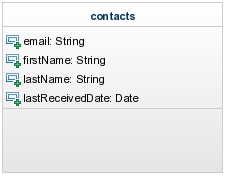
\includegraphics[width=90mm]{img/db_erd.jpg}
\caption{Entity-Relation Diagram for our Data Model \label{db_erd}}
\end{figure}

%\subsubsection{Data dictionary}
%A reference to the data dictionary is provided. The dictionary is maintained in electronic form.

%\section{Functional Model and Description}
%A description of each major software function, along with data flow or class hierarchy (OO) is presented.

%\subsection{Description for Function n}
%A detailed description of each software function is presented. Section 4.1 is repeated for each of n functions.

%\subsubsection{Processing narrative (PSPEC) for function n}
%A processing narrative for function n is presented.

%\subsubsection{Function n flow diagram}
%A diagram showing the flow of information through the function and the transformation it undergoes is presented.

%\subsubsection{Function n interface description}
%A detailed description of the input and output interfaces for the function is presented.

%\subsubsection{Function n transforms}
%A detailed description for each transform (subfunction) for function n is presented. Section 4.1.4 is repeated for each of k transforms.

%Transform k description (processing narrative, PSPEC)

%Transform k interface description

%Transform k lower level flow diagrams

%Transform k interface description

%\subsubsection{Performance Issues}
%Special performance required for the subsystem is specified.

%\subsubsection{Design Constraints}
%Any design constraints that will impact the subsystem are noted.

%\subsection{Software Interface Description}
%The software interface(s)to the outside world is(are) described.

%\subsubsection{External machine interfaces}
%Interfaces to other machines (computers or devices) are described.

%\subsubsection{External system interfaces}
%Interfaces to other systems, products or networks are described.

%\subsubsection{Human interface}
%An overview of any human interfaces to be designed for the software is presented.

%\subsection{Control flow description}
%The control flow for the system is presented with reference to Section 5.0 of this document.

%\section{Behavioral Model and Description}
%A description of the behavior of the software is presented.

%\subsection{Description for software behavior}
%A detailed description of major events and states is presented in this section.

%\subsubsection{Events}
%A listing of events (control, items) that will cause behavioral change within the system is presented.

%\subsubsection{States}
%A listing of states (modes of behavior) that will result as a consequence of events is presented.

%\subsection{State Transition Diagrams}
%Depict the overall behavior of the system.

%\subsection{Control specification (CSPEC)}
%Depict the manner in which control is managed by the software.

%\section{Restrictions, Limitations, and Constraints}
%Special issues which impact the specification, design, or implementation of the software are noted here.

\section{Validation Criteria}
%The approach to software validation is described.

\subsection{Classes of tests}
%The types of tests to be conducted are specified, including as much detail as is possible at this stage. Emphasis here is on black- box testing.
\paragraph{}
We will be running JUnit tests against each iteration of our code to make sure that our program stays consistent.

\paragraph{}
JUnit will be testing all CRUD (Create Update Delete) methods, database interation, data validation, etc methods.

%\subsection{Expected software response}
%The expected results from testing are specified.

%\subsection{Performance bounds}
%Special performance requirements are specified. 

%\section{Appendices}
%Presents information that supplements the Requirements Specification

%\subsection{System traceability matrix}
%A matrix that traces stated software requirements back to the system specification.

%\subsection{Product Strategies}
%If the specification is developed for a product, a description of relevant product strategy is presented here.

%\subsection{Analysis metrics to be used}
%A description of all analysis metrics to be used during the analysis activity is noted here.

%\subsection{Supplementary information (as required)}

\end{document}